% CVPR 2022 Paper Template
% based on the CVPR template provided by Ming-Ming Cheng (https://github.com/MCG-NKU/CVPR_Template)
% modified and extended by Stefan Roth (stefan.roth@NOSPAMtu-darmstadt.de)

\documentclass[10pt,twocolumn,letterpaper]{article}

%%%%%%%%% PAPER TYPE  - PLEASE UPDATE FOR FINAL VERSION
% \usepackage[review]{cvpr}      % To produce the REVIEW version
% \usepackage{cvpr}              % To produce the CAMERA-READY version
\usepackage[pagenumbers]{cvpr} % To force page numbers, e.g. for an arXiv version

% Include other packages here, before hyperref.
\usepackage{subcaption}
\usepackage{graphicx}
\usepackage{amsmath}
\usepackage{amssymb}
\usepackage{booktabs}
\usepackage{array}
\usepackage{listings}
\usepackage{pgffor}
\usepackage{xcolor}
\lstset{
    basicstyle=\ttfamily\small,
    frame=single,
    breaklines=true,
    breakatwhitespace=false,
    columns=fullflexible,
    backgroundcolor=\color{gray!10},
    linewidth=\linewidth,
    % postbreak=\mbox{\textcolor{gray}{$\hookrightarrow$}\space}
}

% It is strongly recommended to use hyperref, especially for the review version.
% hyperref with option pagebackref eases the reviewers' job.
% Please disable hyperref *only* if you encounter grave issues, e.g. with the
% file validation for the camera-ready version.
%
% If you comment hyperref and then uncomment it, you should delete
% ReviewTempalte.aux before re-running LaTeX.
% (Or just hit 'q' on the first LaTeX run, let it finish, and you
%  should be clear).
\usepackage[pagebackref,breaklinks,colorlinks]{hyperref}


% Support for easy cross-referencing
\usepackage[capitalize]{cleveref}
\crefname{section}{Sec.}{Secs.}
\Crefname{section}{Section}{Sections}
\Crefname{table}{Table}{Tables}
\crefname{table}{Tab.}{Tabs.}

\begin{document}

%%%%%%%%% TITLE - PLEASE UPDATE
\title{\LARGE Lab1 Back-Propagation Report \\[0.5em] \large Deep Learning, NYCU}
\author{I-Ting Chu, 111550093}
\maketitle

%%%%%%%%% BODY TEXT
\section{Introduction}
\label{sec:intro}

In this lab, we develop a simple neural network featuring two hidden layers, implemented exclusively using \texttt{NumPy} without the aid of modern deep learning frameworks. This exercise aims to provide a fundamental understanding of the core mechanisms underlying Multi-Layer Perceptrons (MLPs). 

The report is structured as follows: 
Section~\ref{sec:implement} details the implementation of essential components, specifically the neural network architecture and the derivation of the backpropagation algorithm. 
In Section~\ref{sec:exp}, we evaluate the performance of our model on two synthetic datasets—\texttt{linear} and \texttt{XOR}—to verify its functionality through training loss convergence and prediction accuracy analysis. 
Section~\ref{sec:discuss} presents an ablation study investigating the impact of hyper-parameters and architectural choices. 
Finally, Section~\ref{sec:question} discusses the theoretical motivations and mathematical principles behind these design decisions.

%------------------------------------------------------------------------
\section{Implementation Details} \label{sec:implement}

In this section, we detail the modular implementation of our neural network using \texttt{NumPy}. The system is designed with a clear separation between linear transformations, activation functions, and the optimization logic, mirroring the architecture of modern deep learning frameworks.

\subsection{Sigmoid Function}
The Sigmoid function is utilized as the activation layer, especially for the output layer, to squash the input into a range of $(0, 1)$ for binary classification tasks. 
Mathematically, it is defined as:
\[
    \sigma(x) = \frac{1}{1 + e^{-x}}
\]
The gradient of the Sigmoid function can be efficiently computed using its own output: $\sigma'(x) = \sigma(x)(1 - \sigma(x))$. In our implementation, the forward pass caches the output value to accelerate the gradient computation during the backward pass.

\begin{lstlisting}[language=Python, float]
class Sigmoid:
    def __init__(self):
        self.Z = None

    def forward(self, A):
        self.Z = 1.0 / (1.0 + np.exp(-A))
        return self.Z

    def backward(self, dZ):
        local_gradient = self.Z * (1.0 - self.Z)
        dA = dZ * local_gradient  # Chain rule
        return dA
\end{lstlisting}

\subsection{Neural Network Architecture}
The core building block of our architecture is the \texttt{Linear} layer, which performs the affine transformation $Z = XW + b$. We initialize weights using a standard normal distribution and biases as zeros.

\begin{lstlisting}[language=Python]
class Linear:
    def __init__(self, input_dim, output_dim):
        self.input_dim = input_dim
        self.output_dim = output_dim
        self.W = np.random.randn(input_dim, output_dim) 
        self.b = np.zeros((1, output_dim))
        self.dW = np.zeros_like(self.W)
        self.db = np.zeros_like(self.b)

    def forward(self, X):
        self.X = X 
        self.A = X @ self.W + self.b
        return self.A
\end{lstlisting}

Using these blocks, we construct a Multi-Layer Perceptron (MLP) with an input layer (2 features), two hidden layers, and one output layer. The hidden layers also employ \texttt{Sigmoid} activation to introduce non-linearity, enabling the model to learn complex patterns like XOR.

\begin{lstlisting}[language=Python, float]
class NeuralNetwork:
    def __init__(self, h1_dim=4, h2_dim=4):
        self.layers = [
            Linear(2, h1_dim),
            ReLU(),
            Linear(h1_dim, h2_dim),
            Tanh(),
            Linear(h2_dim, 1),
            Sigmoid()
        ]
\end{lstlisting}

\subsection{Backpropagation}
The backpropagation algorithm is implemented by iteratively applying the chain rule from the output layer back to the input layer. For each \texttt{Linear} layer, we compute the gradients for weights ($W$) and biases ($b$) by multiplying the upstream gradient with the local gradient:
\begin{itemize}
    \item $\nabla_W L = X^T \cdot dZ$
    \item $\nabla_b L = \sum dZ$
    \item $\nabla_X L = dZ \cdot W^T$ (passed as the upstream gradient to the previous layer)
\end{itemize}
Inspired by \texttt{Pytorch}, we also implemented a standalone \texttt{SGD} optimizer to decouple the weight update logic from the network layers, facilitating better parameter management through \texttt{step()} and \texttt{zero\_grad()} methods .

\begin{lstlisting}[language=Python]
# Inside Linear Class
def backward(self, dA):
    self.dW += self.X.T @ dA 
    self.db += np.sum(dA, axis=0, keepdims=True)
    dX = dA @ self.W.T 
    return dX

class SGD:
    def __init__(self, parameters, lr=0.01):
        self.parameters = parameters
        self.lr = lr

    def step(self):
        for param in self.parameters:
            param.W -= self.lr * param.dW
            param.b -= self.lr * param.db

    def zero_grad(self):
        for param in self.parameters:
            param.dW.fill(0)
            param.db.fill(0)
\end{lstlisting}

%------------------------------------------------------------------------

\section{Experimental Results} \label{sec:exp}

In this section, we present the performance of our neural network on the \texttt{linear} and \texttt{XOR} datasets. Both experiments were conducted using the same architecture (two hidden layers with Sigmoid activation) but with varying hidden units to accommodate the complexity of the data.

\subsection{Linear Dataset}
For the linear dataset, we utilized a configuration of 4 units for both hidden layers (\texttt{h1\_dim=4, h2\_dim=4}) and a learning rate of 0.1. 

\begin{itemize}
    \item \textbf{Accuracy}: Our model achieved an accuracy of \textbf{1.0 (100\%)} on the testing set, exceeding the 90\% requirement.
    \item \textbf{Learning Curve}: As shown in Figure~\ref{fig:linear_loss}, the loss decreases rapidly within the first 5,000 epochs and stabilizes near zero, indicating successful convergence on the linearly separable data.
\end{itemize}

\begin{figure}[h]
    \centering
    \begin{subfigure}{0.48\textwidth}
        \centering
        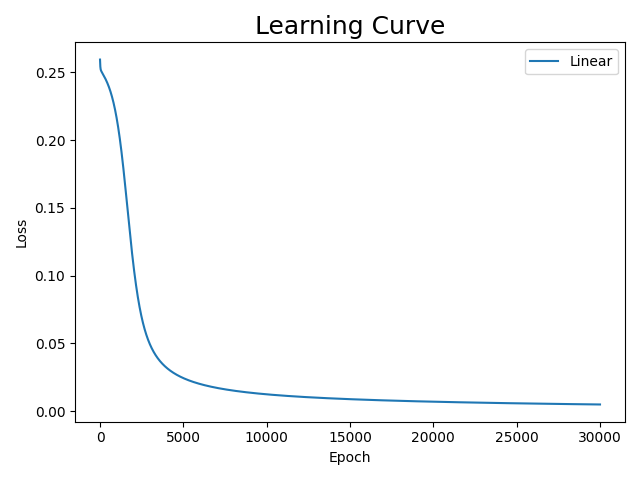
\includegraphics[width=\linewidth]{assets/linear/loss_curve.png}
        \caption{Learning Curve (Linear)}
        \label{fig:linear_loss}
    \end{subfigure}
    \hfill
    \begin{subfigure}{0.48\textwidth}
        \centering
        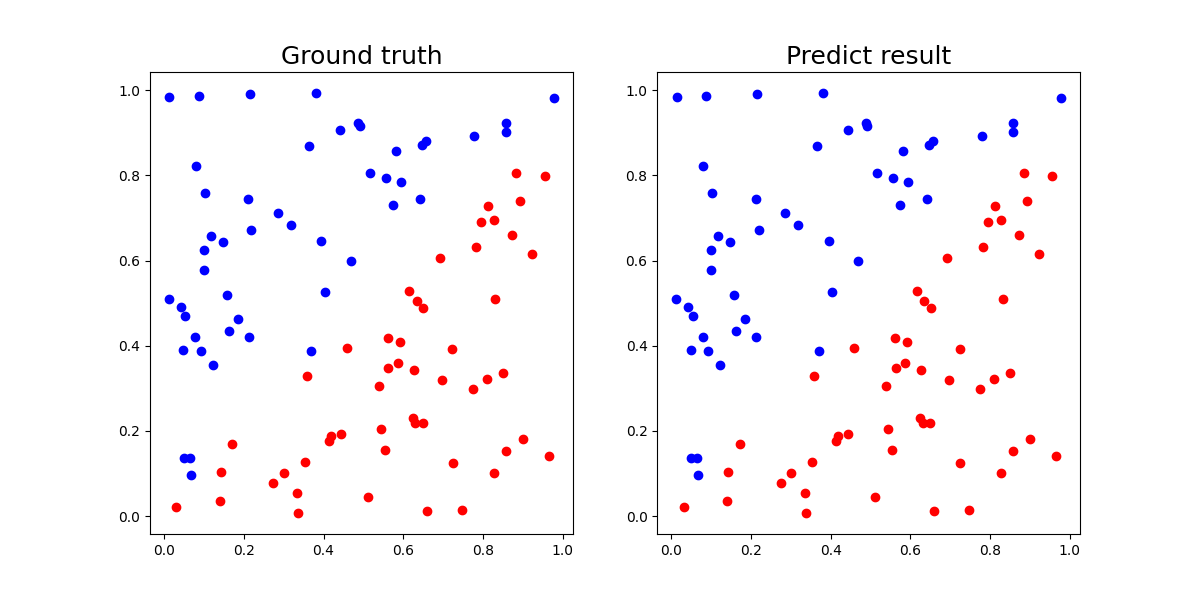
\includegraphics[width=\linewidth]{assets/linear/pred_result.png}
        \caption{Prediction vs. Ground Truth}
        \label{fig:linear_pred}
    \end{subfigure}
    \caption{Experimental results for the Linear dataset.}
\end{figure}

\subsection{XOR Dataset}
The XOR dataset presents a non-linear challenge. To capture the decision boundary, we increased the first hidden layer to 8 units (\texttt{h1\_dim=8, h2\_dim=4}).

\begin{itemize}
    \item \textbf{Accuracy}: Despite the non-linear nature of XOR, the model achieved a perfect accuracy of \textbf{1.0 (100\%)}.
    \item \textbf{Learning Curve}: Figure~\ref{fig:xor_loss} illustrates a distinct ``plateau'' phase around a loss of 0.25 before 15,000 epochs. This behavior is typical for XOR problems as the network searches for the correct non-linear mapping before rapidly converging.
\end{itemize}

\begin{figure}[h]
    \centering
    \begin{subfigure}{0.48\textwidth}
        \centering
        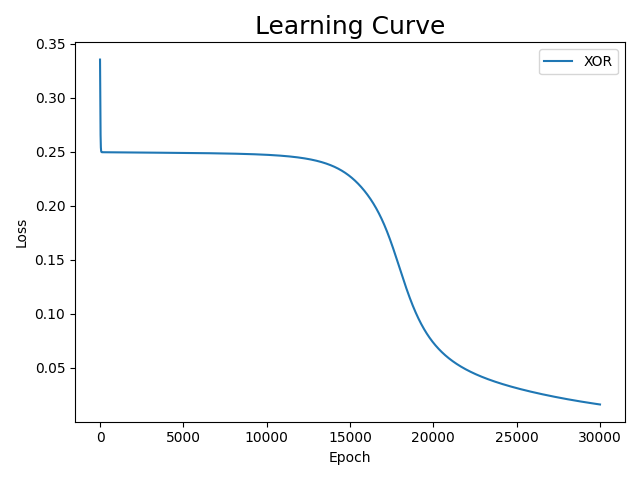
\includegraphics[width=\linewidth]{assets/xor/loss_curve.png}
        \caption{Learning Curve (XOR)}
        \label{fig:xor_loss}
    \end{subfigure}
    \hfill
    \begin{subfigure}{0.48\textwidth}
        \centering
        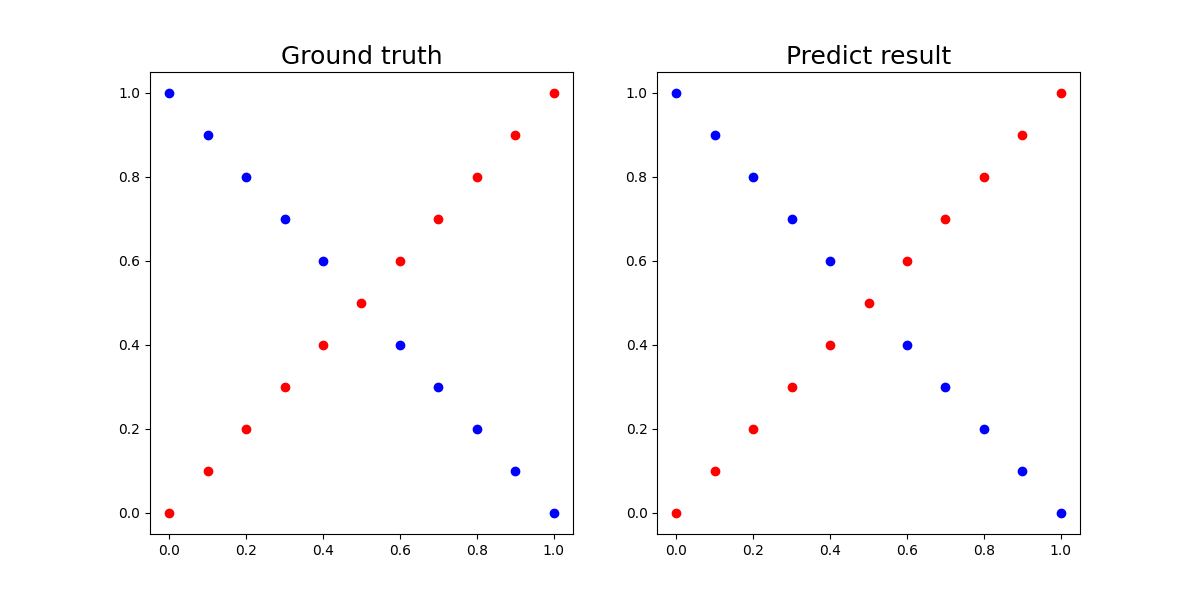
\includegraphics[width=\linewidth]{assets/xor/pred_result.png}
        \caption{Prediction vs. Ground Truth}
        \label{fig:xor_pred}
    \end{subfigure}
    \caption{Experimental results for the XOR dataset.}
\end{figure}

\subsection{Training and Testing Snapshots}
To verify the implementation details, Figure~\ref{fig:snapshots} provides the console output during the training and testing phases for both the \texttt{linear} and \texttt{XOR} datasets. These snapshots confirm the successful decrease in loss values over epochs and the final achievement of 100\% prediction accuracy.

\begin{figure}[h]
    \centering
    % Row 1: Training
    \begin{subfigure}{0.22\textwidth}
        \centering
        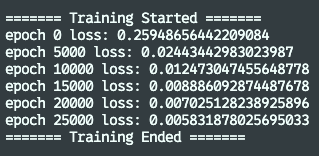
\includegraphics[width=\linewidth]{assets/linear/training_screenshot.png}
        \caption{\texttt{linear} training snapshot}
    \end{subfigure}
    \hfill
    \begin{subfigure}{0.22\textwidth}
        \centering
        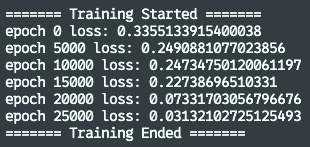
\includegraphics[width=\linewidth]{assets/xor/training_screenshot.png}
        \caption{\texttt{XOR\_easy} training snapshot}
    \end{subfigure}
    \vspace{0.5cm} % Gap between rows

    % Row 2: Testing
    \begin{subfigure}{0.22\textwidth}
        \centering
        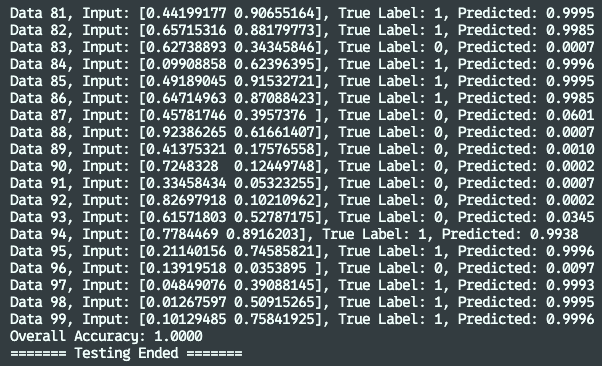
\includegraphics[width=\linewidth]{assets/linear/testing_screenshot.png}
        \caption{\texttt{linear} testing snapshot}
    \end{subfigure}
    \hfill
    \begin{subfigure}{0.22\textwidth}
        \centering
        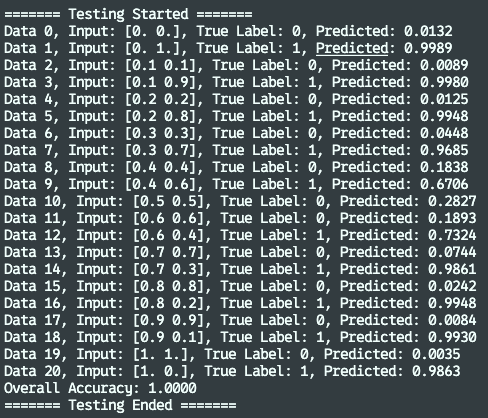
\includegraphics[width=\linewidth]{assets/xor/testing_screenshot.png}
        \caption{\texttt{XOR\_easy} testing snapshot}
    \end{subfigure}
    
    \caption{2x2 Grid of training and testing console snapshots for \texttt{linear} and \texttt{XOR} datasets.}
    \label{fig:snapshots}
\end{figure}

\subsection{Performance Analysis and Comparison}
Comparing the two results, we observe that:
\begin{enumerate}
    \item \textbf{Convergence Speed}: The \texttt{linear} dataset converges significantly faster (approx. 5,000 epochs) compared to the \texttt{XOR} dataset (approx. 25,000 epochs).
    \item \textbf{Model Capacity}: The XOR problem required a larger hidden dimension (\texttt{h1=8}) to successfully find the non-linear decision boundary, whereas the linear problem was solved with fewer parameters.
\end{enumerate}

%------------------------------------------------------------------------

\section{Discussion} \label{sec:discuss}

This section provides an in-depth analysis of the hyper-parameters and architectural design choices that influenced the training efficiency and performance of our modular neural network.

\subsection{Learning Rate Sensitivity Analysis}
We conducted a comprehensive grid search on the learning rate ($lr$) for both datasets, testing values of 0.01, 0.05, 0.1, 0.5, and 1.0. Figure~\ref{fig:lr_tuning_grid} illustrates the impact of these rates on the convergence behavior.

\begin{figure*}[t]
    \centering
    % --- Row 1: Linear Dataset ---
    \begin{subfigure}{0.19\textwidth}
        \centering
        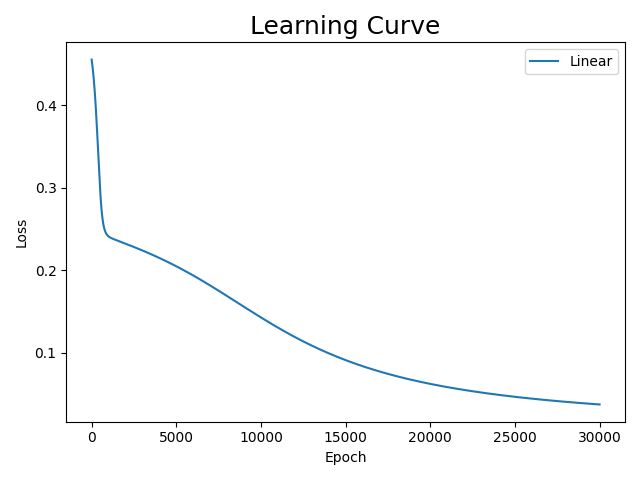
\includegraphics[width=\linewidth]{assets/lr/0.01/linear_loss_curve.png}
        \caption{\texttt{linear}, $lr=0.01$}
    \end{subfigure}
    \hfill
    \begin{subfigure}{0.19\textwidth}
        \centering
        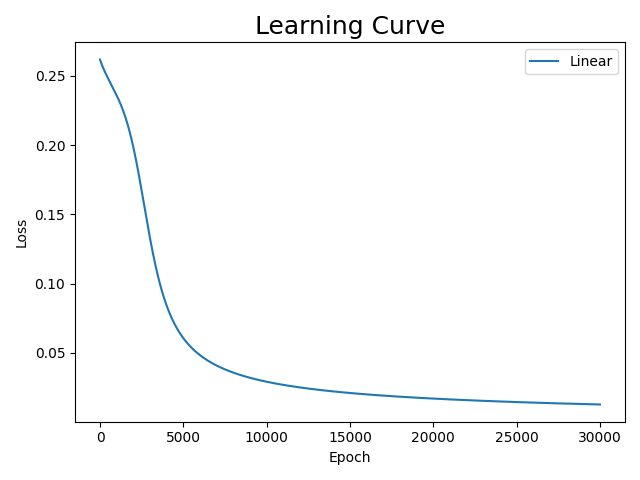
\includegraphics[width=\linewidth]{assets/lr/0.05/linear_loss_curve.png}
        \caption{\texttt{linear}, $lr=0.05$}
    \end{subfigure}
    \hfill
    \begin{subfigure}{0.19\textwidth}
        \centering
        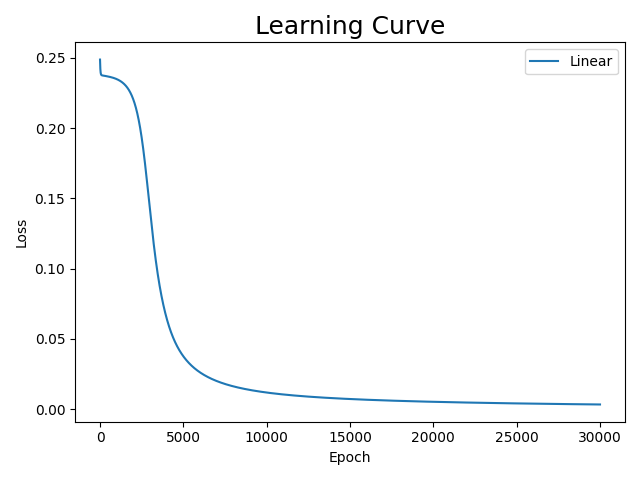
\includegraphics[width=\linewidth]{assets/lr/0.1/linear_loss_curve.png}
        \caption{\texttt{linear}, $lr=0.1$}
    \end{subfigure}
    \hfill
    \begin{subfigure}{0.19\textwidth}
        \centering
        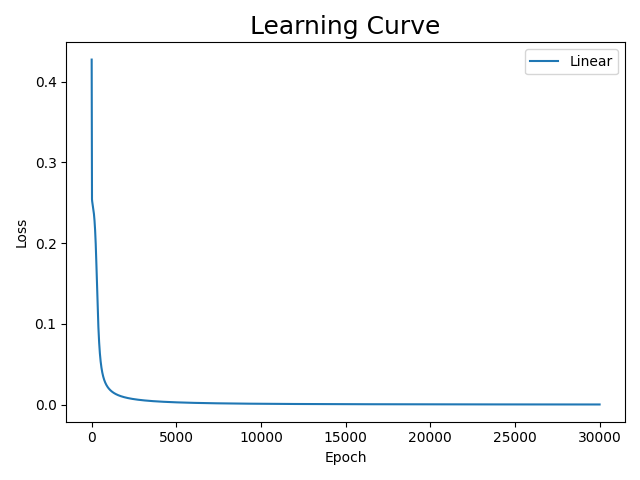
\includegraphics[width=\linewidth]{assets/lr/0.5/linear_loss_curve.png}
        \caption{\texttt{linear}, $lr=0.5$}
    \end{subfigure}
    \hfill
    \begin{subfigure}{0.19\textwidth}
        \centering
        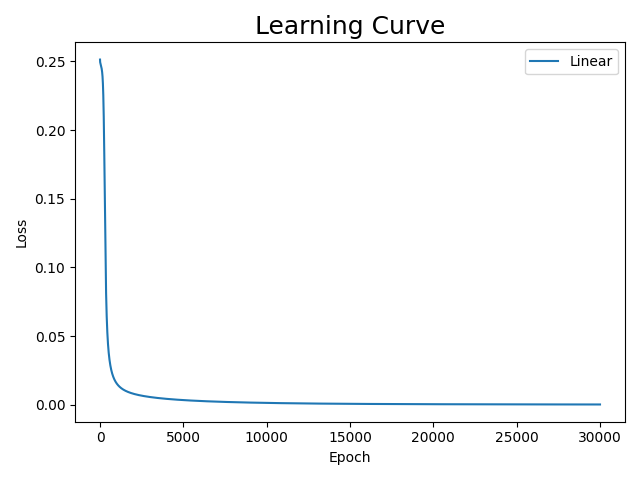
\includegraphics[width=\linewidth]{assets/lr/1/linear_loss_curve.png}
        \caption{\texttt{linear}, $lr=1.0$}
    \end{subfigure}

    \vspace{0.2cm} % Space between rows

    % --- Row 2: XOR Dataset ---
    \begin{subfigure}{0.19\textwidth}
        \centering
        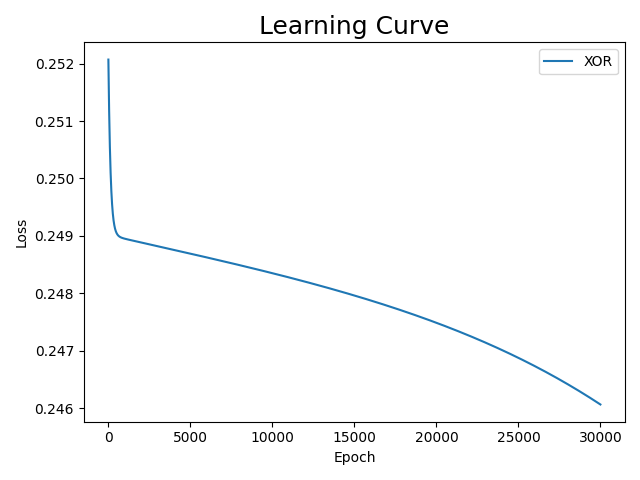
\includegraphics[width=\linewidth]{assets/lr/0.01/xor_loss_curve.png}
        \caption{\texttt{XOR\_easy}, $lr=0.01$}
    \end{subfigure}
    \hfill
    \begin{subfigure}{0.19\textwidth}
        \centering
        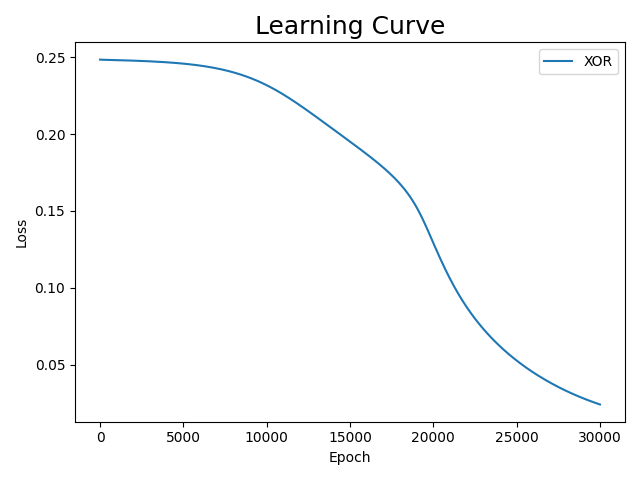
\includegraphics[width=\linewidth]{assets/lr/0.05/xor_loss_curve.png}
        \caption{\texttt{XOR\_easy}, $lr=0.05$}
    \end{subfigure}
    \hfill
    \begin{subfigure}{0.19\textwidth}
        \centering
        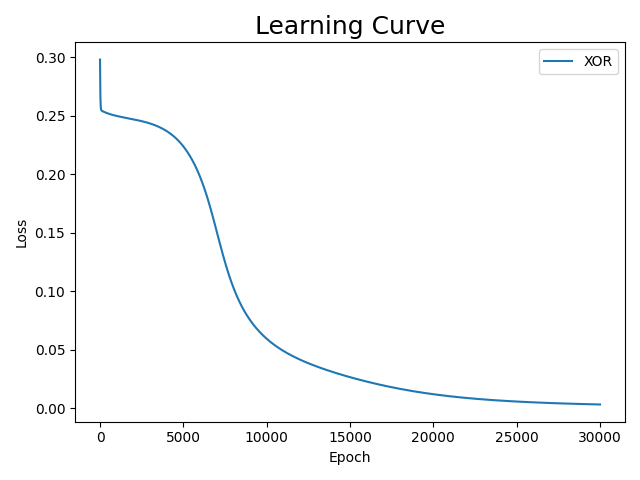
\includegraphics[width=\linewidth]{assets/lr/0.1/xor_loss_curve.png}
        \caption{\texttt{XOR\_easy}, $lr=0.1$}
    \end{subfigure}
    \hfill
    \begin{subfigure}{0.19\textwidth}
        \centering
        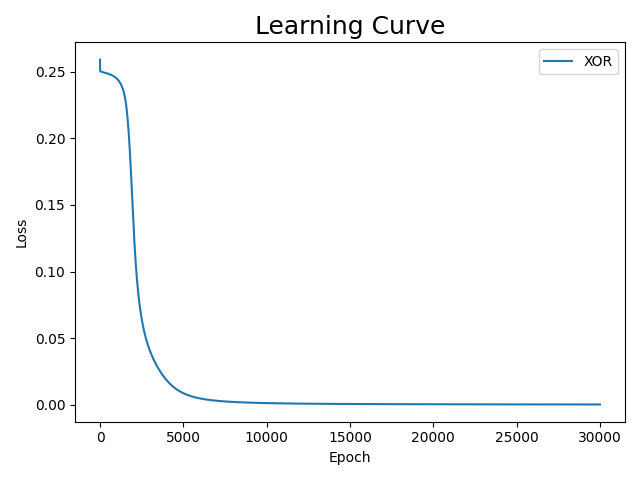
\includegraphics[width=\linewidth]{assets/lr/0.5/xor_loss_curve.png}
        \caption{\texttt{XOR\_easy}, $lr=0.5$}
    \end{subfigure}
    \hfill
    \begin{subfigure}{0.19\textwidth}
        \centering
        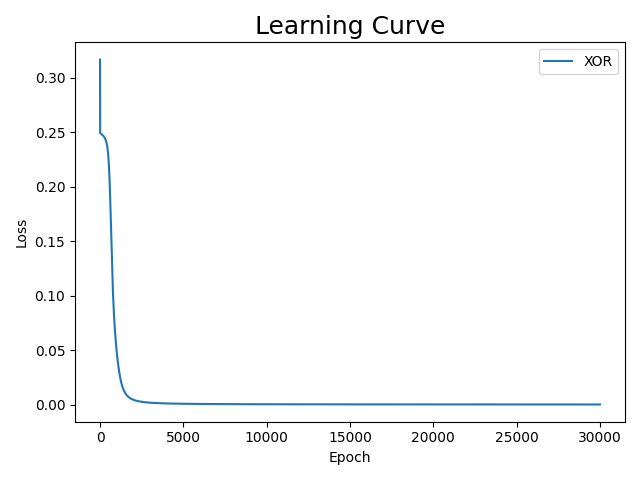
\includegraphics[width=\linewidth]{assets/lr/1/xor_loss_curve.png}
        \caption{\texttt{XOR\_easy}, $lr=1.0$}
    \end{subfigure}
    
    \caption{Learning rate sensitivity analysis. The top row shows the \texttt{linear} dataset, and the bottom row shows the \texttt{XOR\_easy} dataset. Higher learning rates lead to faster convergence, particularly for the non-linear XOR task.}
    \label{fig:lr_tuning_grid}
\end{figure*}

\begin{itemize}
    \item \textbf{Convergence Speed}: There is a direct proportional relationship between the learning rate and the speed of convergence. As shown in our experimental logs, $lr=1.0$ achieves near-zero loss almost instantaneously, while $lr=0.01$ struggles to move past the initial plateau even after 30,000 epochs.
    \item \textbf{Loss Minimization}: For these specific synthetic datasets, higher learning rates did not lead to instability but rather allowed the optimizer to escape local minima or plateaus more effectively. This results in a final loss that closely approaches absolute zero.
\end{itemize}

\subsection{Impact of Hidden Layer Dimensions}
To investigate the relationship between architectural complexity and model performance, we conducted a grid search across various hidden layer sizes ($h1, h2$). Table~\ref{tab:tuning} summarizes the loss and accuracy for both the \texttt{linear} and \texttt{XOR} datasets after 30,000 epochs.

\begin{table}[h]
\centering
\small
\begin{tabular}{cccccc}
\toprule
\textbf{$h1$} & \textbf{$h2$} & \textbf{Lin Loss} & \textbf{Lin Acc} & \textbf{XOR Loss} & \textbf{XOR Acc} \\ \midrule
2 & 2 & 0.008677 & 0.9900 & 0.249104 & 0.5238 \\
2 & 4 & 0.015638 & 0.9800 & 0.015717 & 1.0000 \\
2 & 6 & 0.003117 & 1.0000 & 0.049315 & 0.9524 \\
2 & 8 & 0.006703 & 1.0000 & 0.001865 & 1.0000 \\ \midrule
4 & 2 & 0.003378 & 1.0000 & 0.004150 & 1.0000 \\
4 & 4 & 0.006493 & 1.0000 & 0.001603 & 1.0000 \\
4 & 6 & 0.003547 & 1.0000 & 0.005832 & 1.0000 \\
4 & 8 & 0.005226 & 1.0000 & 0.002150 & 1.0000 \\ \midrule
6 & 2 & 0.006123 & 0.9900 & 0.009770 & 1.0000 \\
6 & 4 & 0.005291 & 1.0000 & 0.002272 & 1.0000 \\
6 & 6 & 0.005912 & 0.9900 & 0.003246 & 1.0000 \\
6 & 8 & 0.012456 & 0.9900 & 0.006426 & 1.0000 \\ \midrule
8 & 2 & 0.004972 & 1.0000 & 0.064458 & 0.9524 \\
8 & 4 & 0.008454 & 1.0000 & 0.001963 & 1.0000 \\
8 & 6 & 0.004548 & 1.0000 & 0.006899 & 1.0000 \\
8 & 8 & 0.005218 & 1.0000 & 0.002215 & 1.0000 \\ \bottomrule
\end{tabular}
\caption{Complete hyperparameter tuning results for hidden unit quantities. The network struggles with the XOR task when either $h1$ or $h2$ creates a severe information bottleneck.}
\label{tab:tuning}
\end{table}

\paragraph{Minimum Configuration for XOR} 
A significant finding is that the smallest configuration ($h1=2, h2=2$) fails to solve the XOR problem, yielding an accuracy of only 52.38\%. This suggests that two hidden units per layer do not provide sufficient degrees of freedom to ``warp'' the 2D input space into a linearly separable representation. However, simply increasing the second hidden layer to 4 units ($h1=2, h2=4$) allows the model to achieve 100\% accuracy, indicating that the network's capacity to resolve non-linearities is highly sensitive to the bottleneck dimension.

\paragraph{Linear Dataset Stability} 
In contrast to the XOR task, the \texttt{linear} dataset proved to be highly robust across all tested dimensions. Even with the minimal $2 \times 2$ architecture, the model achieved 99\% accuracy. This confirms that linearly separable data requires significantly fewer computational resources and a simpler hypothesis space to converge.

\paragraph{Convergence Consistency} 
Configurations with $h1 \ge 4$ consistently achieved 100\% accuracy on both datasets. While increasing the number of units to $8 \times 8$ resulted in slightly lower final loss values, the marginal gain in accuracy was zero, as the problem was already solved. This demonstrates that once a ``threshold capacity'' is reached, further increasing hidden units mainly accelerates convergence rather than improving terminal performance for these synthetic tasks.

\subsection{Performance Without Activation Functions}
To empirically verify the necessity of non-linear activations, we conducted an experiment where the \texttt{Sigmoid} functions in all hidden layers were removed, effectively reducing the MLP to a deep linear network. The comparative results are summarized in Table~\ref{tab:no_activation}.

\begin{table}[h]
\centering
\small
\begin{tabular}{llcc}
\toprule
\textbf{Dataset} & \textbf{Activation} & \textbf{Final Loss} & \textbf{Accuracy} \\ \midrule
\texttt{linear} & With Sigmoid & 0.0087 & 0.9900 \\
\texttt{linear} & Without Sigmoid & 0.0049 & 1.0000 \\ \midrule
\texttt{XOR} & With Sigmoid & 0.0191 & 1.0000 \\
\texttt{XOR} & Without Sigmoid & 0.2494 & 0.5238 \\ \bottomrule
\end{tabular}
\caption{Comparison of performance with and without hidden layer activation functions.}
\label{tab:no_activation}
\end{table}

\paragraph{Observation and Interpretation}
As shown in Table~\ref{tab:no_activation}, the model without activation functions maintains its performance on the \texttt{linear} dataset, achieving 100\% accuracy. However, for the \texttt{XOR\_easy} dataset, the accuracy drops to 52.38\%, which is equivalent to random guessing. 

This behavior is a direct consequence of ``linearity collapse''. Mathematically, a sequence of linear transformations can always be condensed into a single linear transformation:
\[
    Z_n = X \cdot (W_1 W_2 \dots W_n) + b_{total} = X \cdot W_{total} + b_{total}
\]
Since a single linear layer can only define a linear decision boundary (a straight line), it is inherently incapable of separating the XOR classes. Our results confirm that non-linear activation functions are required to ``warp'' the input space, enabling the network to fit non-linear decision boundaries.

%------------------------------------------------------------------------

\section{Questions} \label{sec:question}

In this section, we discuss the theoretical motivations behind neural network design and analyze the empirical findings from our experiments.

\subsection{What is the purpose of activation functions?}
The primary purpose of activation functions is to introduce \textbf{non-linearity} into the network. Without them, any number of linear layers would mathematically collapse into a single linear transformation ($Y = XW_{total} + b_{total}$), limiting the model to solving only linearly separable problems.

\paragraph{Empirical Evidence:} Our experiment in Section~\ref{sec:discuss} demonstrated that removing the \texttt{Sigmoid} activation from hidden layers caused the \texttt{XOR\_easy} accuracy to drop from 1.0 to approximately 0.52 (near-random guessing). This confirms that non-linearity is essential for learning complex decision boundaries like XOR, which cannot be separated by a single straight line.

\subsection{What might happen if the learning rate is too large or too small?}
The learning rate ($lr$) determines the step size taken during gradient descent. 

\begin{itemize}
    \item \textbf{Too Large}: While a high learning rate can accelerate training, it risks ``overshooting'' the global minimum, leading to oscillation or divergence. In our \texttt{linear} dataset trials, $lr=1.0$ converged almost instantly due to the simplicity of the loss surface. However, in more complex landscapes, such a high $lr$ could cause the loss to explode.
    \item \textbf{Too Small}: A learning rate that is too low ensures a stable descent but results in extremely slow convergence. As observed in our tuning results, when $lr=0.01$, the loss for the \texttt{linear} dataset remained high even after 30,000 epochs, indicating that the model was trapped in a plateau and failed to reach the optimum within the given time.
\end{itemize}

\subsection{What is the purpose of weights and biases in a neural network?}
Weights and biases are the fundamental learnable parameters that define the affine transformation $Z = XW + b$.

\begin{itemize}
    \item \textbf{Weights ($W$)}: They control the ``strength'' and ``direction'' of the signal. Geometrically, weights determine the orientation and slope of the decision boundary in the feature space.
    \item \textbf{Biases ($b$)}: They provide an ``offset'' or ``translation'' to the decision boundary. Without a bias term, the decision surface would be forced to pass through the origin $(0,0)$, which significantly restricts the hypothesis space and the model's ability to fit data that is not centered.
\end{itemize}
Together, these parameters allow the model to search for a hyperplane that best separates the target classes.


%%%%%%%%% REFERENCES
% {\small
% \bibliographystyle{ieee_fullname}
% \bibliography{egbib}
% }

\end{document}
